\section{Results}

In this section we will take a look at the results of the optimisation problem.
We look at two differed cloud set-ups for the clouds and wind, a first one will be a system with one big cloud in the center. the second one will have a collection of several smaller clouds.


\section{A first setup}

The results returned by the optimization algorithm  for the first set-up are shown in Figure \ref{fig:badPlot}. 
On this Figure 3 plots are given, one of the actual path, one of the energy stored in the batteries and one of the relative and absolute speed of the plane.
We observe that the flight path nicely avoids the clouds in the centre, while at the same time the plane flies into the sunny area, to charge its batteries. In addition the path starts at the start point and ends at the endpoint. A condition we fed into the solver initially. 
 When taking a closer look at the speed and sun gain plots we observe, that the plane speeds up initially and slows down when it reaches the sunny region that is close to it's destination. A behaviour that we would expect from a good solver, since it leads to higher battery levels if the plane spends more time in the sunny regions.
\begin{figure}[width=15cm]
\begin{minipage}[c][11cm][t]{0.5\textwidth}
  \vspace*{\fill}
  \centering
  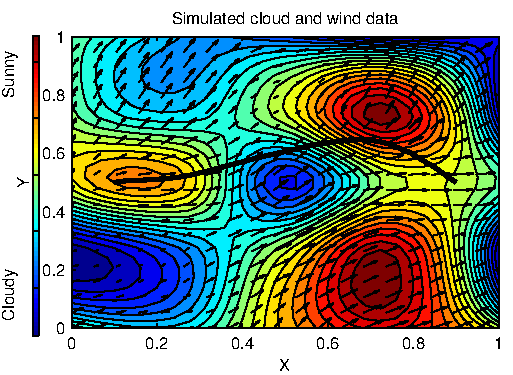
\includegraphics[width=10cm,height=10cm]{../src/plot/fancy1/path}
  \subcaption{test figure one}
  \label{fig:test1}
\end{minipage}%
\begin{minipage}[c][11cm][t]{.5\textwidth}
  \vspace*{\fill}
  \centering
  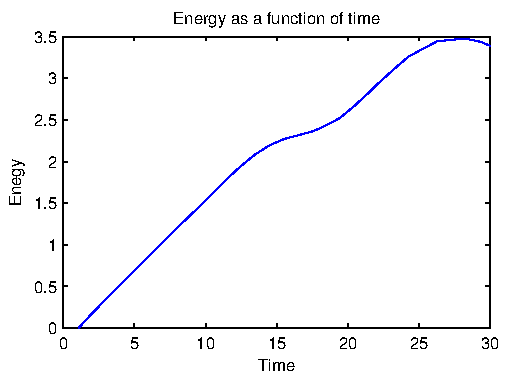
\includegraphics[width=4.5cm,height=4.5cm]{../src/plot/fancy1/Energy}
  \subcaption{test figure two}
  \label{fig:test2}\par\vfill
  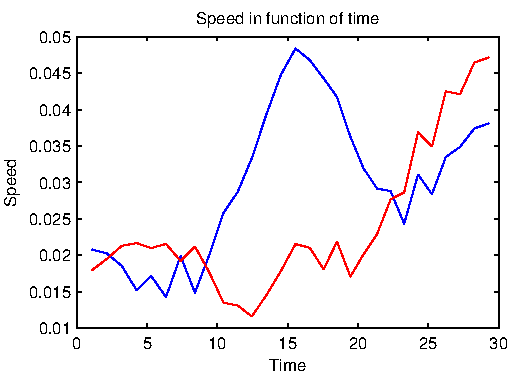
\includegraphics[width=4.5cm,height=4.5cm]{../src/plot/fancy1/speed}
  \subcaption{test figure three}
  \label{fig:test3}
\end{minipage}
\caption{The left plot shows the optimized path for our optimization problem. The speed of the airplane (blue) and the relative speed (red) are shown in the bottom right position. In top the right position we show the amount of energy that's stored in the plane's solar batteries as a function of time. For this setup this function is nearly everywhere increasing.}
\label{fig:badPlot}
\end{figure}

\section{A second setup}


As a second set-up we tried an other set-up for the weather just to look at how the algorithm performers on a complexer problem.
The result of this calculation is given in  Figure \ref{fig:badPlot2}.
Looking at the plots it may look that this solution is not the optimal one, the speed is stil a bid bumpy, especially around time 15.
To calculate this solution we ran let the algorithm run for about an hour, it stopped after 15000 iterations.
The flat spots in the curves is due to to the big steps it is taking at uninteresting places.
When the plane has to manoeuvre very carefully the stepsize gets smaller, this is clearly seen around time 15.



\begin{figure}[width=15cm]
\begin{minipage}[c][11cm][t]{0.5\textwidth}
  \vspace*{\fill}
  \centering
  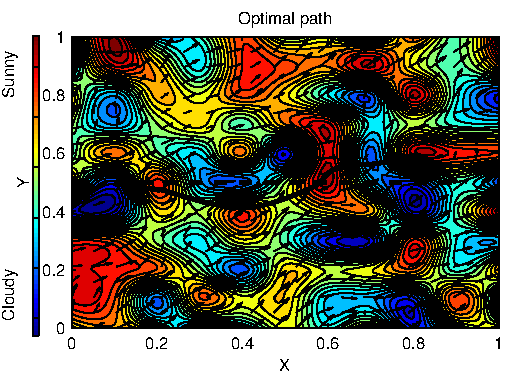
\includegraphics[width=10cm,height=10cm]{../src/plot/fancy2/path}
  \subcaption{test figure one}
  \label{fig:test21}
\end{minipage}%
\begin{minipage}[c][11cm][t]{.5\textwidth}
  \vspace*{\fill}
  \centering
  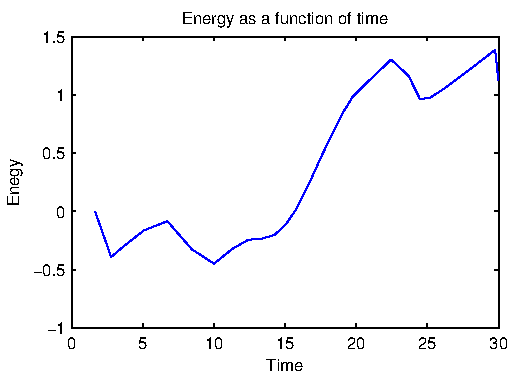
\includegraphics[width=4.5cm,height=4.5cm]{../src/plot/fancy2/Energy}
  \subcaption{test figure two}
  \label{fig:test22}\par\vfill
  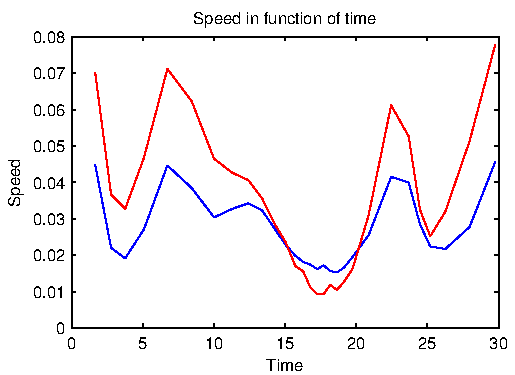
\includegraphics[width=4.5cm,height=4.5cm]{../src/plot/fancy2/speed}
  \subcaption{test figure three}
  \label{fig:test32}
\end{minipage}
\caption{The left plot shows the optimized path for our optimization problem. The speed of the airplane (blue) and the relative speed (red) are shown in the bottom right position. In top the right position we show the amount of energy that's converted in the plane's solar cells as a function of time. The bottom left shows the acceleration as a function of time. The bottom middle plot depicts the energy level in the battery throughout the flight. Finally the bottom right plot depicts the derivative of the cost function.}
\label{fig:badPlot2}
\end{figure}

